\documentclass[12pt, oneside]{article}

\usepackage[letterpaper, scale=0.89, centering]{geometry}
\usepackage{fancyhdr}
\setlength{\parindent}{0em}
\setlength{\parskip}{1em}

\usepackage{tikz}
\usetikzlibrary{automata,positioning,arrows}

\pagestyle{fancy}
\fancyhf{}
\renewcommand{\headrulewidth}{0pt}
\rfoot{\href{https://creativecommons.org/licenses/by-nc-sa/2.0/}{CC BY-NC-SA 2.0} Version \today~(\thepage)}

\usepackage{amssymb,amsmath,pifont,amsfonts,comment,enumerate,enumitem}
\usepackage{currfile,xstring,hyperref,tabularx,graphicx,wasysym}
\usepackage[labelformat=empty]{caption}
\usepackage{xcolor}
\usepackage{multicol,multirow,array,listings,tabularx,lastpage,textcomp,booktabs}

% NOTE(joe): This environment is credit @pnpo (https://tex.stackexchange.com/a/218450)
\lstnewenvironment{algorithm}[1][] %defines the algorithm listing environment
{   
    \lstset{ %this is the stype
        mathescape=true,
        frame=tB,
        numbers=left, 
        numberstyle=\tiny,
        basicstyle=\rmfamily\scriptsize, 
        keywordstyle=\color{black}\bfseries,
        keywords={,procedure, div, for, to, input, output, return, datatype, function, in, if, else, foreach, while, begin, end, }
        numbers=left,
        xleftmargin=.04\textwidth,
        #1
    }
}
{}

\newcommand\abs[1]{\lvert~#1~\rvert}
\newcommand{\st}{\mid}

\newcommand{\cmark}{\ding{51}}
\newcommand{\xmark}{\ding{55}}


\begin{document}
\begin{flushright}
    \StrBefore{\currfilename}{.}
\end{flushright}

\section*{Before we start}
If you or someone you know is suffering from food and/or housing insecurities 
there are UCSD resources here to help:

Basic Needs Office: \href{https://basicneeds.ucsd.edu/}{https://basicneeds.ucsd.edu/}

Triton Food Pantry (in the old Student Center)
is free and anonymous, and includes produce: 

\href{https://www.facebook.com/tritonfoodpantry/}{https://www.facebook.com/tritonfoodpantry/}

Mutual Aid UCSD: \href{https://mutualaiducsd.wordpress.com/}{https://mutualaiducsd.wordpress.com/}

If you find yourself in an uncomfortable situation, ask for help. 
We are committed to upholding University policies regarding nondiscrimination, sexual violence and sexual harassment.

Counseling and Psychological Services (CAPS) at 858 5343755 or \href{http://caps.ucsd.edu}{http://caps.ucsd.edu}


OPHD at (858) 534-8298, ophd@ucsd.edu , \href{http://ophd.ucsd.edu}{http://ophd.ucsd.edu}. 
CARE at Sexual Assault Resource Center at 858 5345793 sarc@ucsd.edu \href{http://care.ucsd.edu}{http://care.ucsd.edu}

\subsection*{Spring quarter philosophy}
Spring 2022 is a transition quarter so please be patient with us as we do our best 
to serve the needs of all students while adhering to the university guidelines. 
First and foremost is the health and safety of everyone.  
Please do not come to class if you are sick or even think you might be sick.
Please reach out (minnes@eng.ucsd.edu) if you need support with extenuating circumstances.

Masks are required in class. All students who attend class must also be fully vaccinated against COVID-19
unless they have a university-approved exemption.
Campus policy requires masks and daily ``symptom screeners" for everyone and we expect all students 
to follow these rules. 


\newpage
Welcome to CSE 105: Introduction to Theory of Computation in Spring 2022!

\section*{Themes and applications for CSE 105}
\begin{itemize}
\item {\bf Technical skepticism}: Know, select and apply appropriate computing knowledge and problem-solving techniques. 
Reason about computation and systems. 
Use mathematical techniques to solve problems. 
Determine appropriate conceptual tools to apply to new situations. 
Know when tools do not apply and try different approaches. 
Critically analyze and evaluate candidate solutions.
\item {\bf Multiple representations}: Understand, guide, shape impact of computing on society/the world. 
Connect the role of Theory CS classes to other applications (in undergraduate CS curriculum and beyond). 
Model problems using appropriate mathematical concepts.
Clearly and unambiguously communicate computational ideas using appropriate formalism. 
Translate across levels of abstraction.
\end{itemize}

{\bf Applications}: Numbers (how to represent them and use them in Computer Science), 
Recommendation systems and their roots in machine learning (with applications like Netflix),
``Under the hood" of computers (circuits, pixel color representation, data structures),
Codes and information (secret message sharing and error correction),
Bioinformatics algorithms and genomics (DNA and RNA).

\section*{Introductions}
Class website: \href{http://cseweb.ucsd.edu/classes/fa21/cse20-a}{http://cseweb.ucsd.edu/classes/fa21/cse20-a}

{\bf Pro-tip}: the URL structure is your map to finding your course website for other CSE classes.

{\bf Pro-tip}: you can use MATH109 to replace CSE20 for prerequisites and other requirements.

Instructor: Prof. Mia Minnes {\tiny{"Minnes" rhymes with Guinness}}, minnes@eng.ucsd.edu, 
\href{http://cseweb.ucsd.edu/~minnes}{http://cseweb.ucsd.edu/~minnes}

Our team: Four TAs and 10 tutors + all of you

Fill in contact info for students around you, if you'd like:
\vspace{50pt}


On a typical week: {\bf MWF} Lectures + review quizzes, {\bf T} HW due, {\bf W} Discussion, office hours, Piazza. 
Project parts will be due some weeks.

All dates are on \href{https://canvas.ucsd.edu/}{Canvas (click for link)} and details are on
 \href{https://theory-cs.github.io/website/overview_calendar.html}{course calendar (click for link)}.


\newpage
\section*{Monday March 28}

%! app: Regular Languages
%! outcome: Define decision problem

The CSE 105 vocabulary and notation build on discrete
math and introduction to proofs classes.  Some of the conventions may 
be a bit different so we'll draw your attention to them.

For consistency, we will use the notation from this class' textbook\footnote{Page references are to 
the 3rd edition (International) of Sipser's Introduction to the Theory of Computation,
available through various sources for under \$30. You may be able to 
opt in to purchase a digital copy through Canvas. Copies of the book are also available 
for those who can't access the book
to borrow from the course instructor, while supplies last (minnes@ucsd.edu)}.

These definitions are on pages 3, 4, 6, 13, 14, 53.

\begin{center}
    \begin{tabular}{|p{2.6in}cp{3.5in}|}
    \hline 
    {\bf Term} & {\bf Typical symbol} & {\bf Meaning} \\
     & or {\bf Notation} & \\
    \hline
    && \\
    Alphabet & $\Sigma$, $\Gamma$ & A non-empty finite set	 \\
    Symbol over $\Sigma$  & $\sigma$, $b$, $x$ & An element of the alphabet $\Sigma$\\ 
    String over $\Sigma$  &	$u$, $v$, $w$ & A finite list of symbols from $\Sigma$\\
    (The) empty string &$\varepsilon$ & The (only) string of length $0$\\
    The set of all strings over $\Sigma$ & $\Sigma^*$ & The collection of all possible strings formed from symbols from $\Sigma$ \\ 
    (Some) language over $\Sigma$& $L$ & (Some) set of strings over $\Sigma$ \\ 
    (The) empty language &$\emptyset$ & The empty set, i.e. the set that has no strings (and no other elements either)\\
    && \\
    \hline
    && \\
    The power set of a set $X$ &$\mathcal{P}(X)$ & The set of all subsets of $X$ \\
    (The set of) natural numbers &$\mathcal{N}$ & The set of positive integers \\ 
    (Some) finite set & & The empty set or a set whose distinct elements can be counted by a natural number\\
    (Some) infinite set & & A set that is not finite.\\ 
    &&\\
    \hline
    && \\
    Reverse of a string $w$ & $w^\mathcal{R}$  & write $w$  in  the opposite order, if $w = w_1 \cdots  w_n$ then $w^\mathcal{R} = w_n \cdots  w_1$. Note: $\varepsilon^\mathcal{R} = \varepsilon$\\
    Concatenating strings $x$ and $y$ & $xy$ &  take $x = x_1 \cdots x_m$, $y=y_1 \cdots y_n$ and form $xy = x_1 \cdots x_m y_1 \cdots y_n$\\
    String $z$ is a substring of string $w$ & & there are strings $u,v$ such that $w = uzv$\\
    String $x$ is a prefix of string $y$ & & there is a string $z$ such that $y = xz$ \\
    String $x$ is a proper prefix of string $y$ & & $x$ is a prefix of $y$ and $x \neq y$\\
    && \\
    \hline
    &&\\
    Shortlex order, also known as string order over alphabet $\Sigma$ & & Order strings over  $\Sigma$ first by length and then according to the dictionary order, assuming symbols in $\Sigma$  have an ordering.\\ \hline
    \end{tabular}
\end{center}

\vfill
    

Write out in words the meaning of the symbols below: 
\[
    \{ a,b, c\}
\]

\phantom{The set whose elements are $a$, $b$, and $c$}

\[
    | \{a, b, a \} | = 2
\]

\phantom{The number of elements in the set $\{a,b,a\}$ is $2$.}

\[
    | aba | = 3
\]

\phantom{The length of the string $aba$ is $3$.}

\[
    (a, 3, 2, b, b)
\]

\phantom{The $5$-tuple whose first components is $a$, second component 
is $3$, third component is $2$, fourth component is $b$, and fifth component is $b$.}


{\it Circle the correct choice}:

A {\bf string} over an alphabet $\Sigma$ is \underline{~~an element of $\Sigma^*$ ~~ OR ~~ a subset of $\Sigma^*$}.
    
A {\bf language} over an alphabet $\Sigma$ is \underline{~~an element of $\Sigma^*$ ~~ OR ~~ a subset of $\Sigma^*$}.


{\it Extra examples for practice:}

With $\Sigma_1 = \{0,1\}$ and $\Sigma_2 = \{a,b,c,d,e,f,g,h,i,j,k,l,m,n,o,p,q,r,s,t,u,v,w,x,y,z\}$  and $\Gamma = \{0,1,x,y,z\}$

An example of a string of length 3 over $\Sigma_1$ is \underline{\phantom{ $000$} \hspace{0.2in}}

An example of  a string of length 1 over $\Sigma_2$ is  \underline{\phantom{ $k$} \hspace{0.2in}}

The number of distinct strings of length 2 over $\Gamma$ is  \underline{\phantom{ $25$} \hspace{0.2in}}

An example of a language over $\Sigma_1$ of size $1$ is  \underline{\phantom{ $ \{ \varepsilon \} $} \hspace{0.2in}}

An example of an infinite language over $\Sigma_1$ is  \underline{\phantom{ $\Sigma^*$} \hspace{0.2in}}
    
An example of  a finite language over $\Gamma$ is  \underline{\phantom{ $\{ 0, x \}$} \hspace{0.2in}}
    
{\bf True} or {\bf False}: $\varepsilon \in \Sigma_1$

{\bf True} or {\bf False}: $\varepsilon$ is  a string over $\Sigma_1$

{\bf True} or {\bf False}: $\varepsilon$ is a language over $\Sigma_1$

{\bf True} or {\bf False}: $\varepsilon$ is a prefix of some string over  $\Sigma_1$

{\bf True} or {\bf False}: There is a string over $\Sigma_1$ that is a proper prefix of $\varepsilon$
    

The first five strings over $\Sigma_1$ in string order, using the ordering $0 <  1$: \vfill
    
The first five strings over $\Sigma_2$ in string order, using the usual alphabetical ordering for single letters: \vfill

    
\newpage
\subsection*{Review: Week 1 Monday}
\begin{enumerate}
\item Please complete the beginning of the quarter survey \href{https://forms.gle/gvibFnNixxqcWbaU8}{https://forms.gle/gvibFnNixxqcWbaU8}
\item We want you to be familiar with class policies and procedures so you are ready to have a successful quarter. 
Please take a look at the class website http://cseweb.ucsd.edu/classes/fa21/cse20-a
and answer the questions about it on \href{http://gradescope.com}{Gradescope}.
\end{enumerate}

{\bf Pre class reading for next time}: Figure 1.4, Definition 1.5

\newpage
\subsection*{Week 1 Wednesday}

\begin{center}
    \begin{tabular}{|ll|}
    \hline
    Alphabet e.g. $\Sigma$, $\Gamma$ & 	non-empty finite set	 \\
    Symbol over $\Sigma$  & element of alphabet $\Sigma$\\
    String over $\Sigma$  &	finite list of symbols from $\Sigma$\\
    Language over $\Sigma$& set of strings over $\Sigma$ \\
    Empty set $\emptyset$ & the empty language\\
    Regular expression over $\Sigma$ e.g. $R$& syntactic expression built up recursively \\
    Language described by $R$,  $L(R)$ & set of strings matching pattern given by 
    regular expression\\
    \hline
    {\it Pages 3, 4, 13, 14, 64, 65}& \\
    \hline
    \end{tabular}
    \end{center}
    
    
    For the following True/False questions assume the alphabet is $\Sigma =  \{a,b,c\}$:
    
    \begin{center}
    \begin{tabular}{lcc}
    $a  \in L(a \cup b \cup c)$ & True & False \\
    $ab  \in L(~ (a \cup b)^*  ~)$ & True & False \\
    $ba \in L( ~ a^* b^* ~)$ & True & False \\
    $\varepsilon  \in L(a \cup b \cup c)$ & True & False \\
    $\varepsilon  \in L(~ (a \cup b)^*  ~)$ & True & False \\
    $\varepsilon \in L( ~ a^* b^* ~)$ & True & False \\
    \end{tabular}
    \end{center}
    
    
    
    \begin{center}
    \begin{tabular}{|ll|}
    \hline
    & \\
    Deterministic finite automaton & $M = (Q, \Sigma, \delta, q_0, F)$ \\
    Finite set of states $Q$  & Can  be labelled by any collection  of distinct names. Default: $q0, q1, \ldots$  \\
    Alphabet $\Sigma$ &   Each input to the automaton is a string over  $\Sigma$. \\
    Transition function $\delta$ &  Gives the next state based on current state of machine next input symbol\\
    Start state $q_0$ & Element of $Q$.  Each computation of the machine starts at the  start  state.\\
    Accept (final) states $F$ & $F \subseteq  Q$. Used to flag if the machine accepts or rejects
    an input string.\\
    Computation & The computation of a machine on an input string is a sequence of states \\
    &  in the machine,  starting with the initial state, determined by transitions \\
    & of the machine as it reads successive input symbols.
    \\
    $M$ accepts the input string & The computation of $M$ on the input string ends in an
    accept state.\\
    $M$ rejects the input string & The computation of $M$ on the input string ends in a
    nonaccept state.\\
    Language of $M$, $L(M)$ & The set of  all strings that  are each accepted by the machine $M$.\\
    aka language recognized by $M$ & \\
    & \\
    \hline
    {\it Pages 34-36}& \\
    \hline
    \end{tabular}
    \end{center}
    
    
    What is {\bf finite} about a deterministic finite automaton? (Select all that apply)
    \begin{itemize}
    \item The size of the machine (number of states, number of arrows)
    \item The number of strings that are accepted by the machine
    \item The length of the computations of the machine
    \end{itemize}
    
    
    
    
    \begin{figure}[h]
       \centering
       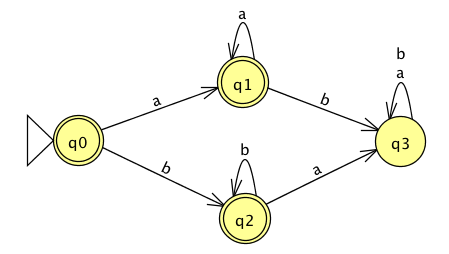
\includegraphics[width=3in]{../../resources/machines/Lect2DFA1.png} 
    \end{figure}
    
    The formal definition of this DFA is
    
    \vspace{100pt}
    
    
    \begin{center}
    \begin{tabular}{lcc}
    {\bf Input string} & {\bf Result}: this string is \ldots    & \\
    \hline
    $a$ & accepted by the DFA & rejected by the DFA \\
    $aa$ & accepted by the DFA & rejected by the DFA \\
    $ab$ & accepted by the DFA & rejected by the DFA \\
    $ba$ & accepted by the DFA & rejected by the DFA \\
    $bb$ & accepted by the DFA & rejected by the DFA \\
    $\varepsilon$ & accepted by the DFA & rejected by the DFA \\
    \end{tabular}
    \end{center}
    
    The language recognized by this DFA is
    
    
    \begin{figure}[h]
       \centering
       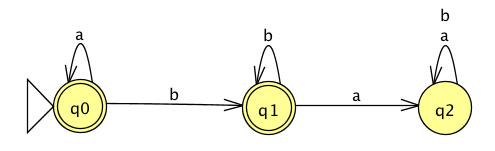
\includegraphics[width=3in]{../../resources/machines/Lect2DFA2.png} 
    \end{figure}
    
    
    
    The language recognized by this DFA is
    
    
    
    \begin{figure}[h]
       \centering
       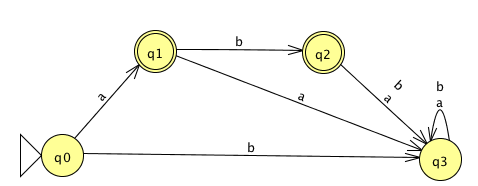
\includegraphics[width=3in]{../../resources/machines/Lect2DFA3.png} 
    \end{figure}
    
    
    The language recognized by this DFA is
    
    

\end{document}